% IEEE conference paper — ICDSG 2026: 4--6 pages including figures, tables, references
% (see https://www.icdsg.org/2026/). Double-blind: no names/affiliations in the review PDF.
%
% Build: pdflatex main && bibtex main && pdflatex main && pdflatex main
% Long draft: main_long.tex
%
% After acceptance / camera-ready: comment out the next line (or set \icdsgreviewfalse).
\newif\ificdsgreview
\icdsgreviewtrue

\documentclass[conference]{IEEEtran}
\IEEEoverridecommandlockouts

\usepackage{amsmath,amssymb}
\usepackage{booktabs}
\usepackage{graphicx}
\usepackage{dblfloatfix}
\usepackage[hidelinks]{hyperref}
\usepackage{xcolor}

\hypersetup{pdfborder={0 0 0}}
\ificdsgreview
\hypersetup{pdfauthor={}}
\else
\hypersetup{pdfauthor={Areg Khachatryan}}
\fi

% Slightly roomier tables without changing IEEE fonts.
\newcommand{\tablestretch}{\renewcommand{\arraystretch}{1.08}}

\title{Short-Term $PM_{2.5}$ Forecasting in Yerevan:\\
Comparing Statistical and Machine Learning Models}

\ificdsgreview
\author{%
\IEEEauthorblockN{Anonymous author(s)}%
\IEEEauthorblockA{%
\textit{Author identities withheld for double-blind review (ICDSG 2026)}%
}%
}
\else
\author{%
\IEEEauthorblockN{Areg Khachatryan}%
\IEEEauthorblockA{%
American University of Armenia\\
Yerevan, Armenia}%
}
\fi

\begin{document}
\maketitle
\begin{abstract}
We compare parsimonious time-series models (AR, SARIMA) to machine learning (gradient boosting, DeepAR) for hourly $PM_{2.5}$ in Yerevan, Armenia, at horizons 1--24\,h, with strict chronological splits, walk-forward robustness, block-bootstrap confidence intervals for MAE, and Diebold--Mariano tests with HAC variance. While AR(24) provides the best performance for spatially aggregated city and district metrics---including district-weighted MAE 3.66\,$\mu$g/m$^3$ versus persistence at 3.82\,$\mu$g/m$^3$ ($h{=}1$)---simple Persistence remains the most robust baseline for individual station-level forecasting. Tuned ensembles improve over ridge but do not beat strong linear autoregression at 1\,h on the primary test window. DeepAR (MAE 26.31\,$\mu$g/m$^3$ at 1\,h) under a deliberately minimal, ``vanilla'' configuration performs poorly, illustrating that complex sequence models are not informative without task-specific scaling and tuning in high-variance urban series.
\ificdsgreview
Implementation details are omitted for double-blind review and will be documented in camera-ready materials.
\else
Code and data instructions accompany the project repository.
\fi
\end{abstract}

\begin{IEEEkeywords}
Air quality, $PM_{2.5}$, forecasting, Diebold--Mariano test, machine learning, time series.
\end{IEEEkeywords}

\section{Introduction}

Fine particulate matter ($PM_{2.5}$) is a major urban health risk and a regulated indicator in many jurisdictions~\cite{world2021who}. Short-horizon forecasts support public alerts, routing advice, and communication when concentrations rise quickly. Yerevan, the capital of Armenia, exhibits strong winter pollution episodes tied to space heating, topography, and meteorology; at the same time, open national monitoring supports reproducible modeling from public feeds.

Machine learning is widely applied to air quality prediction~\cite{shao2020predictions}, yet low-order autoregressive and seasonal ARIMA structures often remain strong baselines when persistence is high and samples are limited~\cite{box2015time,hyndman2021forecasting}. Fair comparison therefore requires leakage control (no future covariates in features), temporal robustness beyond a single split, and uncertainty for point metrics, not only leaderboard MAE.

Validation hygiene matters: leakage and single-fold leaderboards inflate ML gains~\cite{hyndman2021forecasting}, and spatial smoothing changes error scales, so scores must name their geographic support. We therefore prioritize chronological splits and walk-forward re-fitting to reduce ``lucky split'' bias that is common in air-quality ML comparisons.

We ask: (i)~when linear models outperform ML at 1--24\,h; (ii)~how city, district, and station aggregation changes rankings; (iii)~whether tuned boosting and a sequence model (DeepAR) change conclusions; (iv)~whether rankings hold under walk-forward refitting. We report frozen AR coefficients after training, HAC Diebold--Mariano tests~\cite{diebold1995comparing,harvey1997testing}, circular block bootstrap for MAE uncertainty, and a modular, scripted pipeline for replication.

\textbf{Contributions.} (1)~Preprocessing with controlled imputation and strictly past-only features. (2)~A benchmark zoo: baselines, AR(24), SARIMA, ridge, forests, boosted trees (Hyperopt-tuned), inverse-MAE and average ensembles, and DeepAR. (3)~Walk-forward evaluation with SARIMA re-estimated each fold. (4)~Spatial comparison of weighted test MAE across aggregation levels.

\section{Related work}

Forecast comparison tests~\cite{diebold1995comparing,harvey1997testing} motivate paired testing on loss differentials rather than informal gap inspection: when errors are serially correlated, standard normal critical values for mean error gaps are misleading, whereas HAC variance estimates align nominal size better in hourly environmental series. Environmental ML surveys~\cite{shao2020predictions} document widespread nonlinear modeling while often leaving classical time-series baselines under-tuned or mis-aligned with the forecast horizon; a common pattern is to compare a deep model to a default ARIMA rather than to a long-lag AR that matches the effective memory of the target.

Direct multi-step estimation~\cite{marcellino2006comparison} matches our per-horizon supervised learners. Local context appears in~\cite{auaair2025yerevan}; aggregating stations to districts or a city mean changes noise and can reorder models, which matters for mapped indicators versus sensor-level analytics.

\section{Data and methods}

\subsection{Data, stations, and spatial targets}
Open hourly air quality from the national portal is aligned to a regular clock; the primary target is city-average $PM_{2.5}$ ($\mu$g/m$^3$). Covariates include $PM_{10}$, temperature, pressure, and humidity when complete on the modeling grid. The district inventory lists 205 unique monitoring stations that enter the city mean. Figure~\ref{fig:stations} plots every geocoded site used in the analysis; district labels report site counts that \emph{sum to 205}, matching the inventory total. Overlapping markers at identical coordinates can make the network appear visually sparser than the true count. Stations map to administrative districts (eleven of twelve districts represented; one district has no assigned sites). District-level series are district means over member stations; station-level analyses weight units by inverse historical missingness so that informative sites contribute more to aggregates of errors.

Figure~\ref{fig:stations} situates the monitoring network geographically; Section~\ref{sec:results} reports accuracy on the city mean and on district- and station-weighted targets.

\begin{figure}[!t]
\centering
\includegraphics[width=\columnwidth]{../images/stations_map_lonlat.png}
\caption{Geocoded monitoring stations ($n{=}205$; district legend $n$ sum to 205) used in this study, colored by district (metadata coordinates).}
\label{fig:stations}
\end{figure}

\subsection{Preprocessing, gaps, and features}
Short gaps in $PM_{2.5}$ use time-local interpolation; medium gaps use hour-of-day medians learned on training data; residual covariate holes use capped fills. The modeling table is restricted to rows with listwise-complete features after imputation. Feature construction uses only information available at forecast time $t$: lags up to 72\,h, rolling means and standard deviations over 6--48\,h, low-order Fourier seasonality, calendar and heating-season indicators, and optional meteorology interactions. $PM_{2.5}$ inputs are winsorized at the training 99.5th percentile to limit leverage from spikes.

Figure~\ref{fig:acf} shows autocorrelation structure on the training window for the city mean: strong short-lag dependence motivates AR(24) as a substantive baseline rather than a strawman, and periodic spikes at 24\,h multiples reflect the diurnal cycle that seasonal na\"{\i}ve rules target.

\begin{figure}[!t]
\centering
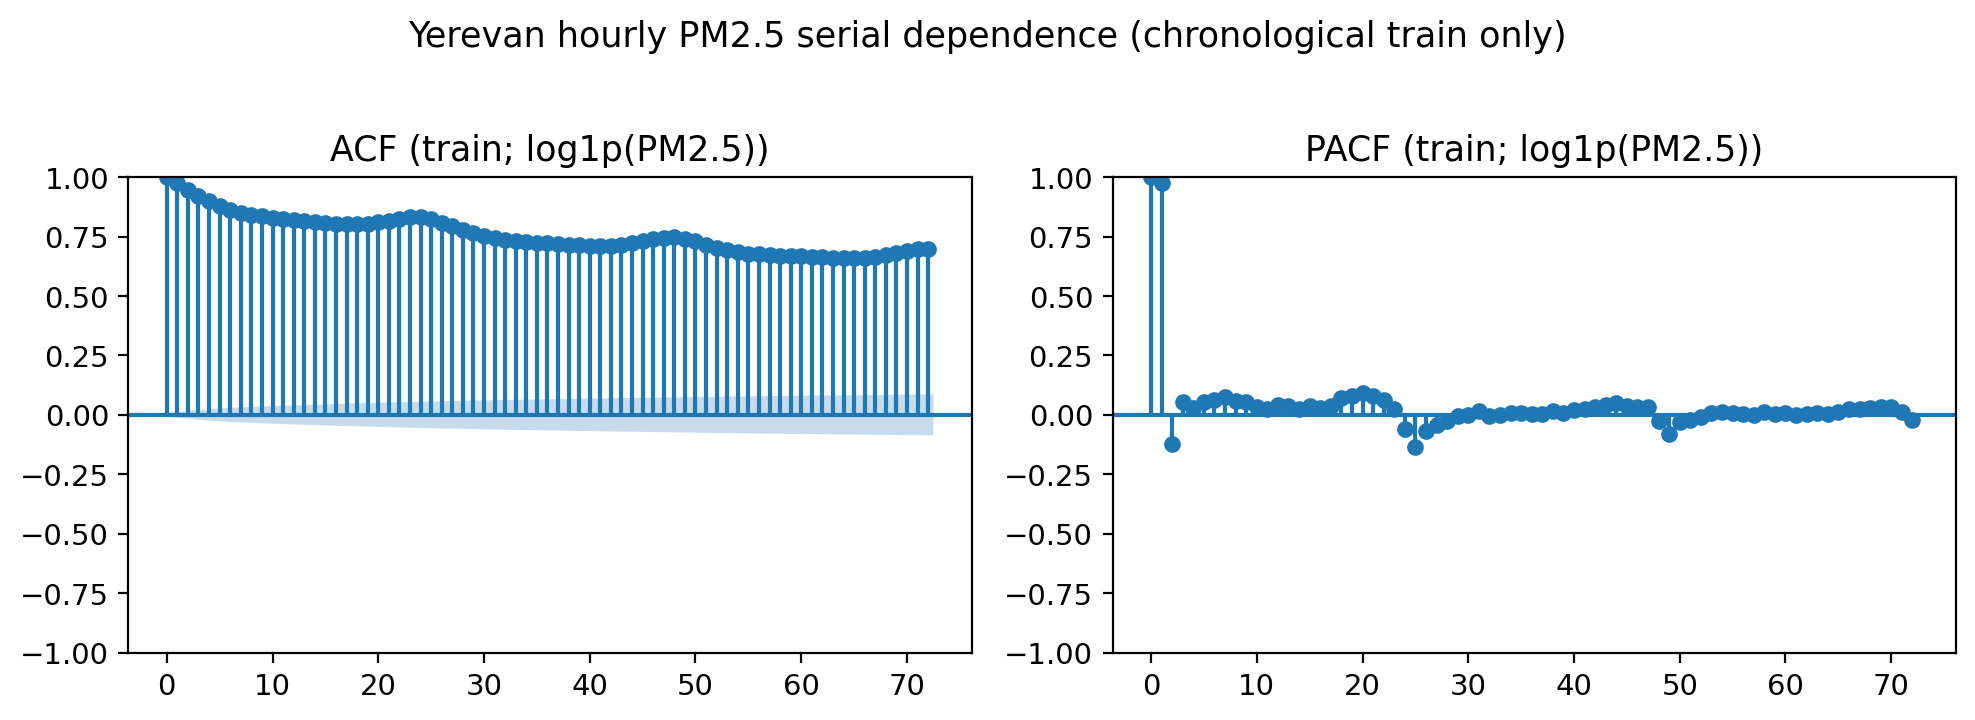
\includegraphics[width=0.92\columnwidth]{../images/acf_pacf_train.png}
\caption{ACF and PACF of training-window city-mean $PM_{2.5}$ (hourly).}
\label{fig:acf}
\end{figure}

\subsection{Model families}
\textbf{Baselines.} Persistence ($\hat y_{t+h}=y_t$), seasonal naive with 24\,h lag, and a 24\,h trailing mean.

\textbf{AR(24).} Univariate autoregression with fixed order 24 on the target scale being modeled:
\begin{equation}
y_t = \sum_{i=1}^{24} \phi_i\, y_{t-i} + \varepsilon_t .
\end{equation}
After joint least squares on the training window, coefficients $\{\phi_i\}$ are frozen and applied on validation and test (no recursive re-fit each hour).

\textbf{SARIMA.} Seasonal ARIMA $(2,1,2)\times(1,0,0)_{24}$ estimated on a trailing 8{,}760\,h ($\approx$one year) window before each forecast origin for scalability and recency; multi-step point forecasts use the fitted state for $h{=}1$ in the main table, with walk-forward re-estimation each fold.

\textbf{Supervised ML.} Ridge regression on the engineered lag library; random forest, XGBoost, and LightGBM with validation-tuned hyperparameters (10 Hyperopt trials in the reported run). Ensembles combine the top three validation models by inverse MAE or simple average.

\textbf{DeepAR.} We include a \emph{vanilla} DeepAR baseline (NeuralForecast) with library-default-style training and scaling, intended not as a best-effort neural competitor but to demonstrate the risk of deploying complex sequence models without task-specific preprocessing, hyperparameter search, and stability checks. The resulting 1\,h MAE (Table~\ref{tab:main}) is far above classical baselines and should be read as a cautionary negative result rather than a fair ceiling for deep forecasting.

\subsection{Splits, walk-forward, and testing}
The primary experiment uses a 70\%/15\%/15\% chronological split on the modeling table: training through 2023-12-29, validation through 2025-01-14, and test through 2026-01-31 (illustrative dates from the frozen export). An expanding walk-forward scheme advances by roughly one month, refitting all models each fold; tree methods reuse validation-tuned hyperparameters for computational stability. This re-fit protocol is a deliberate guard against optimistic one-window results: if ranking changes sharply across folds, we treat single-split wins as unstable.

\subsection{Metrics and inference}
Point metrics are MAE, RMSE, and $R^2$ on the test slice. Supervised models are trained for horizons $\mathcal{H}=\{1,2,3,4,6,12,24\}$ (direct multi-step). Uncertainty for MAE uses a circular block bootstrap (2000 draws) with block length chosen to respect diurnal structure.

For paired comparison of absolute errors $\{|e_{t,h}^{(A)}|,|e_{t,h}^{(B)}|\}$, Diebold--Mariano uses mean loss differential $\bar d$ with a heteroskedasticity- and autocorrelation-consistent (HAC) variance estimator; we report the standard normal statistic and two-sided $p$-values~\cite{diebold1995comparing,harvey1997testing}. Only a small set of pairs is tested to limit multiplicity.

\section{Results}
\label{sec:results}

\subsection{City-mean accuracy at 1~h}
Table~\ref{tab:main} ranks models on the primary city-average target (all MAE values in $\mu$g/m$^3$). At $h{=}1$, AR(24) achieves MAE 2.41, Persistence 2.75, SARIMA 4.38, and Ridge 4.66---values mirrored in Table~\ref{tab:hz} (Table~III) and the city row of Table~\ref{tab:spat} (Table~IV). AR(24) leads overall, followed by persistence and inverse-MAE ensembles; gradient boosting improves markedly with tuning but does not close the gap to AR(24). SARIMA and Ridge sit mid-pack; seasonal naive and DeepAR illustrate failure modes (misaligned seasonality and a minimal sequence baseline, respectively). The poor performance of DeepAR (MAE 26.31\,$\mu$g/m$^3$) highlights the sensitivity of global sequence models to the high-variance, localized spikes characteristic of Yerevan's winter $PM_{2.5}$ pollution.

\begin{table*}[!t]
\centering
\tablestretch
\footnotesize
\caption{Test performance at horizon $h=1$\,h, city-average $PM_{2.5}$ ($\mu$g/m$^3$).}
\label{tab:main}
\input{../paper/tables/ieee/main_results_tabular.tex}
\end{table*}

\subsection{Bootstrap intervals and Diebold--Mariano tests}
Table~\ref{tab:bootdm} pairs block-bootstrap MAE intervals with DM tests for representative comparisons at $h{=}1$. Intervals for AR(24) and persistence do not overlap those for ridge. On $n{=}9{,}178$ hourly test rows (HAC lag 25), the two-sided Diebold--Mariano $p$-values are $p{<}0.001$ for AR(24) versus persistence (DM${=}8.74$) and $p{<}0.001$ for AR(24) versus ridge (DM${=}17.38$); thus the city-mean MAE advantage for AR(24) is statistically discernible at conventional levels, not merely a numerical tie under serial dependence.

\begin{table*}[!t]
\centering
\footnotesize
\caption{Left: block-bootstrap 95\% MAE intervals. Right: Diebold--Mariano tests on absolute loss (illustrative pairs, $h{=}1$).}
\label{tab:bootdm}
\begin{minipage}[t]{0.49\textwidth}\centering
\tablestretch
\textbf{(a)} Bootstrap MAE 95\% CIs\par\vspace{0.4em}
\input{../paper/tables/ieee/bootstrap_tabular.tex}
\end{minipage}\hfill
\begin{minipage}[t]{0.49\textwidth}\centering
\tablestretch
\textbf{(b)} Diebold--Mariano\par\vspace{0.4em}
\input{../paper/tables/ieee/dm_tabular.tex}
\end{minipage}
\end{table*}

\subsection{Horizons beyond one step}
Figure~\ref{fig:mae} (Figure~3 in the compiled layout) traces MAE across horizons: persistence error grows faster than supervised models, while AR(24) remains strongest at short lags. Table~\ref{tab:hz} (Table~III) gives a compact numeric view for selected models; Ridge reaches MAE 9.52\,$\mu$g/m$^3$ at 24\,h, and SARIMA is reported at 1\,h only (4.38\,$\mu$g/m$^3$) because our production path emphasizes single-step state forecasts for that specification.

\begin{figure*}[!t]
\centering
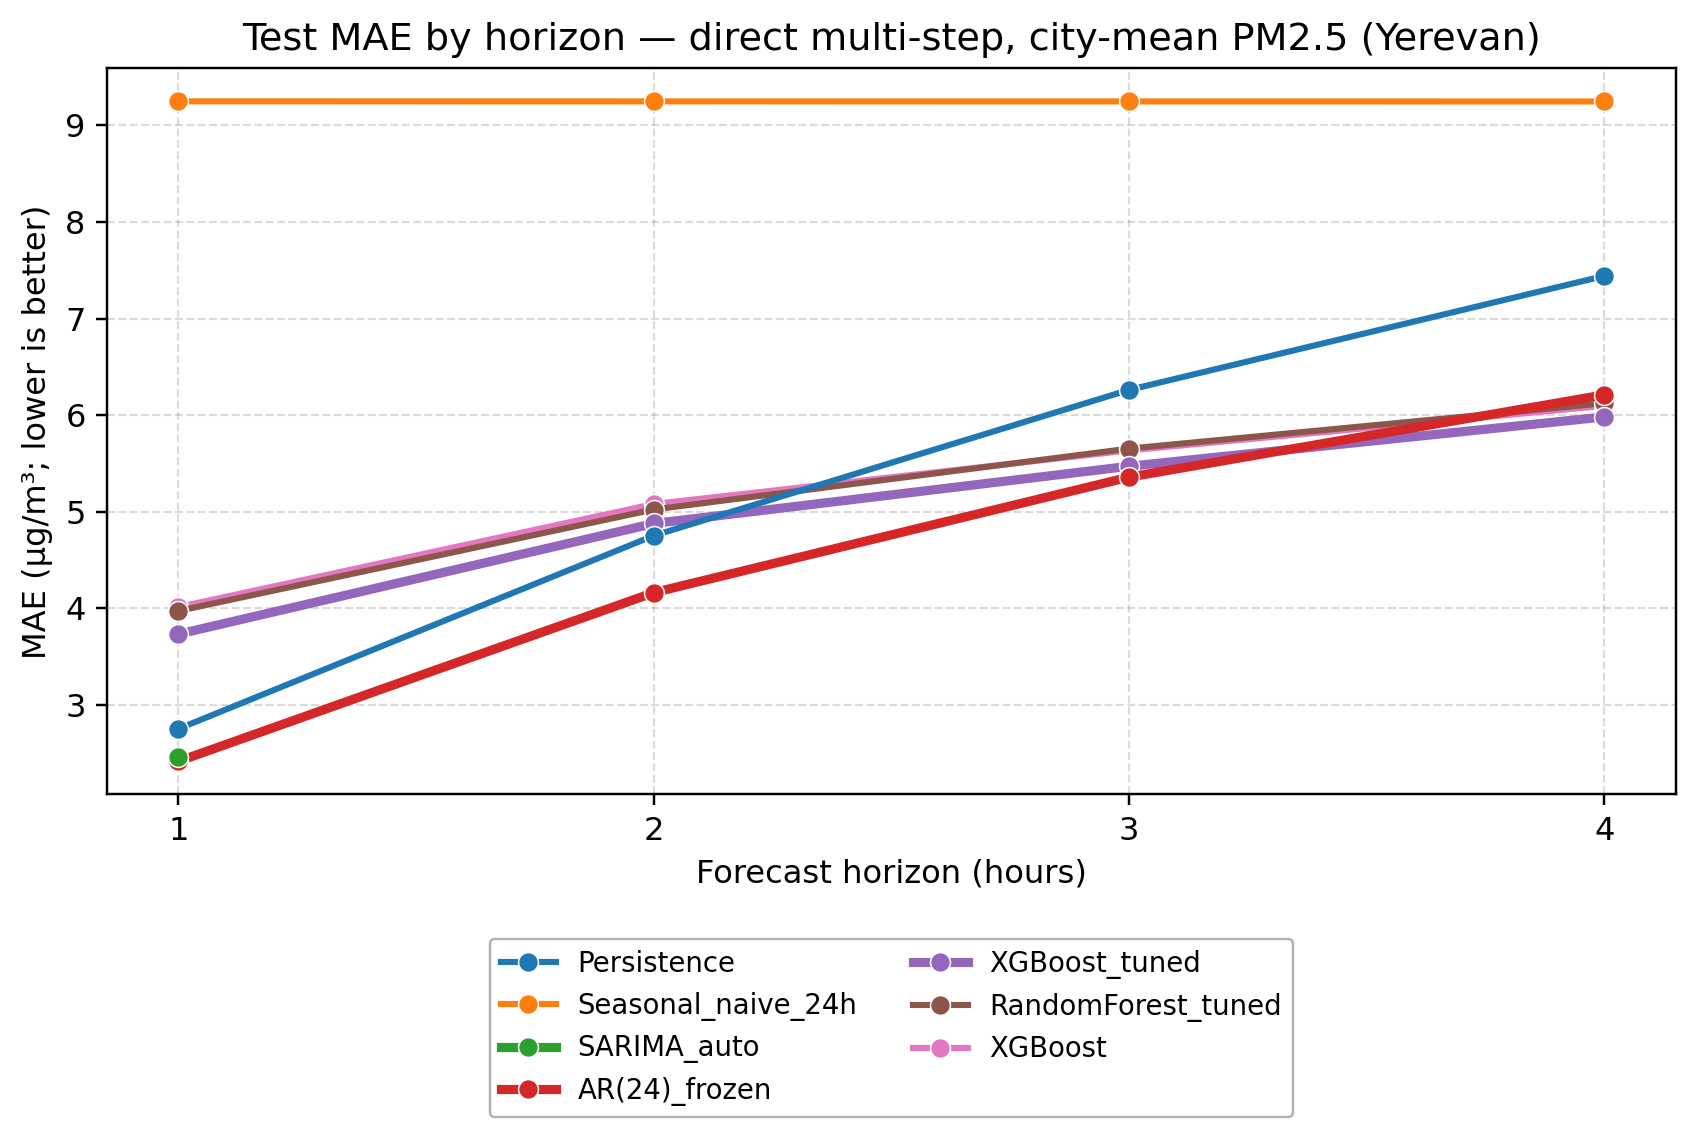
\includegraphics[width=0.94\textwidth]{../images/mae_by_horizon.png}
\caption{Test MAE by forecast horizon for city-mean $PM_{2.5}$ (direct multi-step supervised learners; AR/SARIMA paths per implementation).}
\label{fig:mae}
\end{figure*}

\begin{table*}[!t]
\centering
\tablestretch
\footnotesize
\caption{Test MAE ($\mu$g/m$^3$) by horizon for selected models. Dashes: horizon not reported for SARIMA in this configuration.}
\label{tab:hz}
\input{../paper/tables/ieee/mae_by_horizon_tabular.tex}
\end{table*}

\subsection{Spatial aggregation and walk-forward stability}
Spatial aggregation tells a coherent story at $h{=}1$ (MAE in $\mu$g/m$^3$). On the city mean, AR(24) is best at 2.41\,$\mu$g/m$^3$ (Table~\ref{tab:spat}, Table~IV). On the district-weighted target (Table~\ref{tab:spat}: district means with inverse-missingness weights on units), AR(24) remains best at \textbf{3.66}\,$\mu$g/m$^3$, ahead of persistence at \textbf{3.82}\,$\mu$g/m$^3$ (i.e., still below $\approx$4.0 but materially above the city-scale errors). At station-sample weighting, persistence wins at 9.91\,$\mu$g/m$^3$ versus AR(24) at 10.10\,$\mu$g/m$^3$ (Table~\ref{tab:spat}), so finer spatial support reverses the ranking even though AR(24) still wins on smoothed city and district aggregates. Figure~\ref{fig:spatialmae} and Figure~\ref{fig:wf} summarize 1-hour ranking and fold stability: mean ranks remain consistent with the single split---AR(24) leads among compared models on aggregated targets; SARIMA ranks between tuned gradient boosting and ridge on 1\,h city MAE (Table~\ref{tab:main}, Figure~\ref{fig:spatialmae}) but exhibits higher fold-to-fold variance than AR(24) in walk-forward evaluation.

\begin{table}[!t]
\centering
\tablestretch
\footnotesize
\caption{Top-two models by spatial aggregation level ($h{=}1$, $\mu$g/m$^3$; district and station targets are missingness-weighted).}
\label{tab:spat}
\input{../paper/tables/ieee/spatial_tabular.tex}
\end{table}

\begin{figure*}[!t]
\centering
\begin{minipage}[t]{0.49\textwidth}
\centering
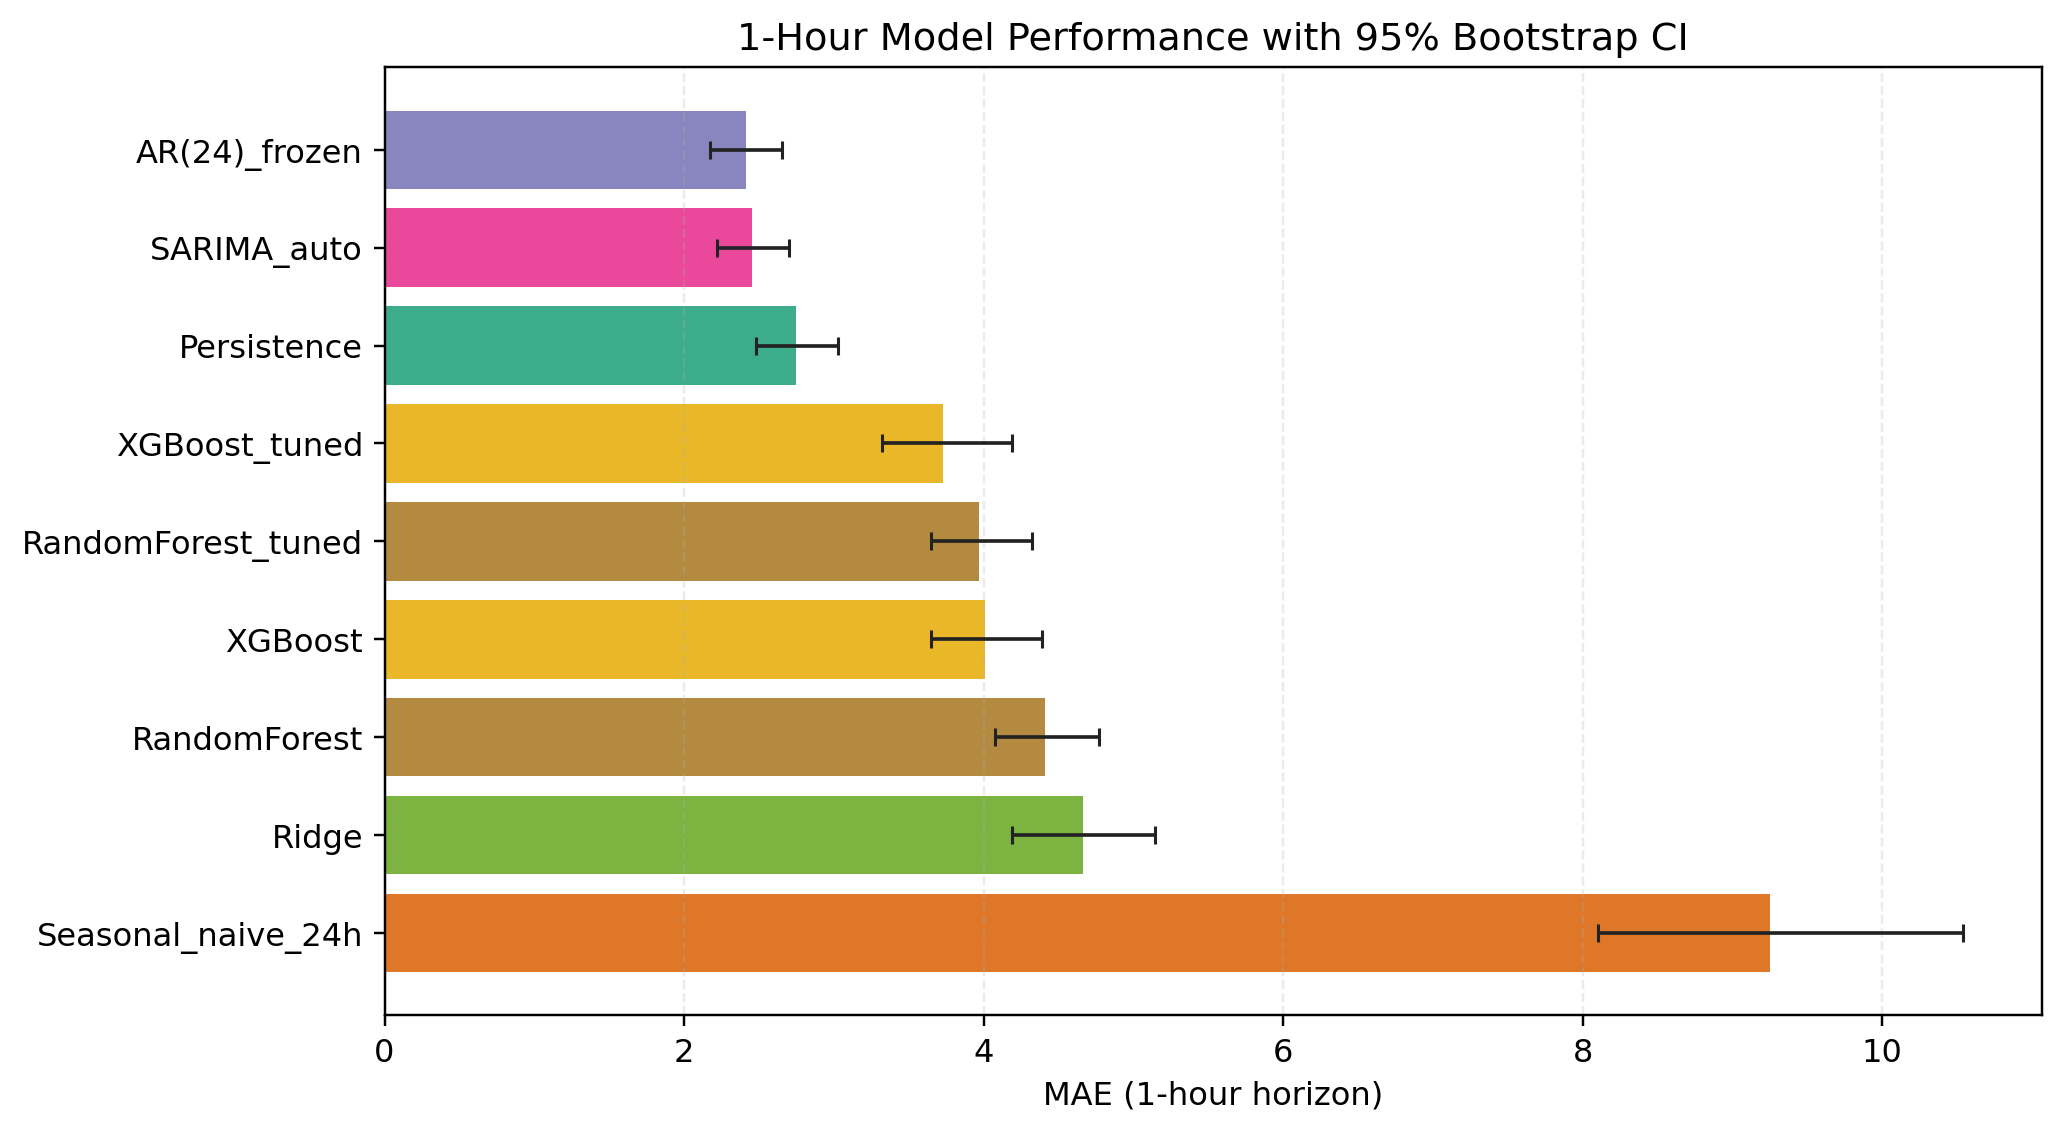
\includegraphics[width=\textwidth]{../images/model_performance_1h_ci.png}
\end{minipage}\hfill
\begin{minipage}[t]{0.49\textwidth}
\centering
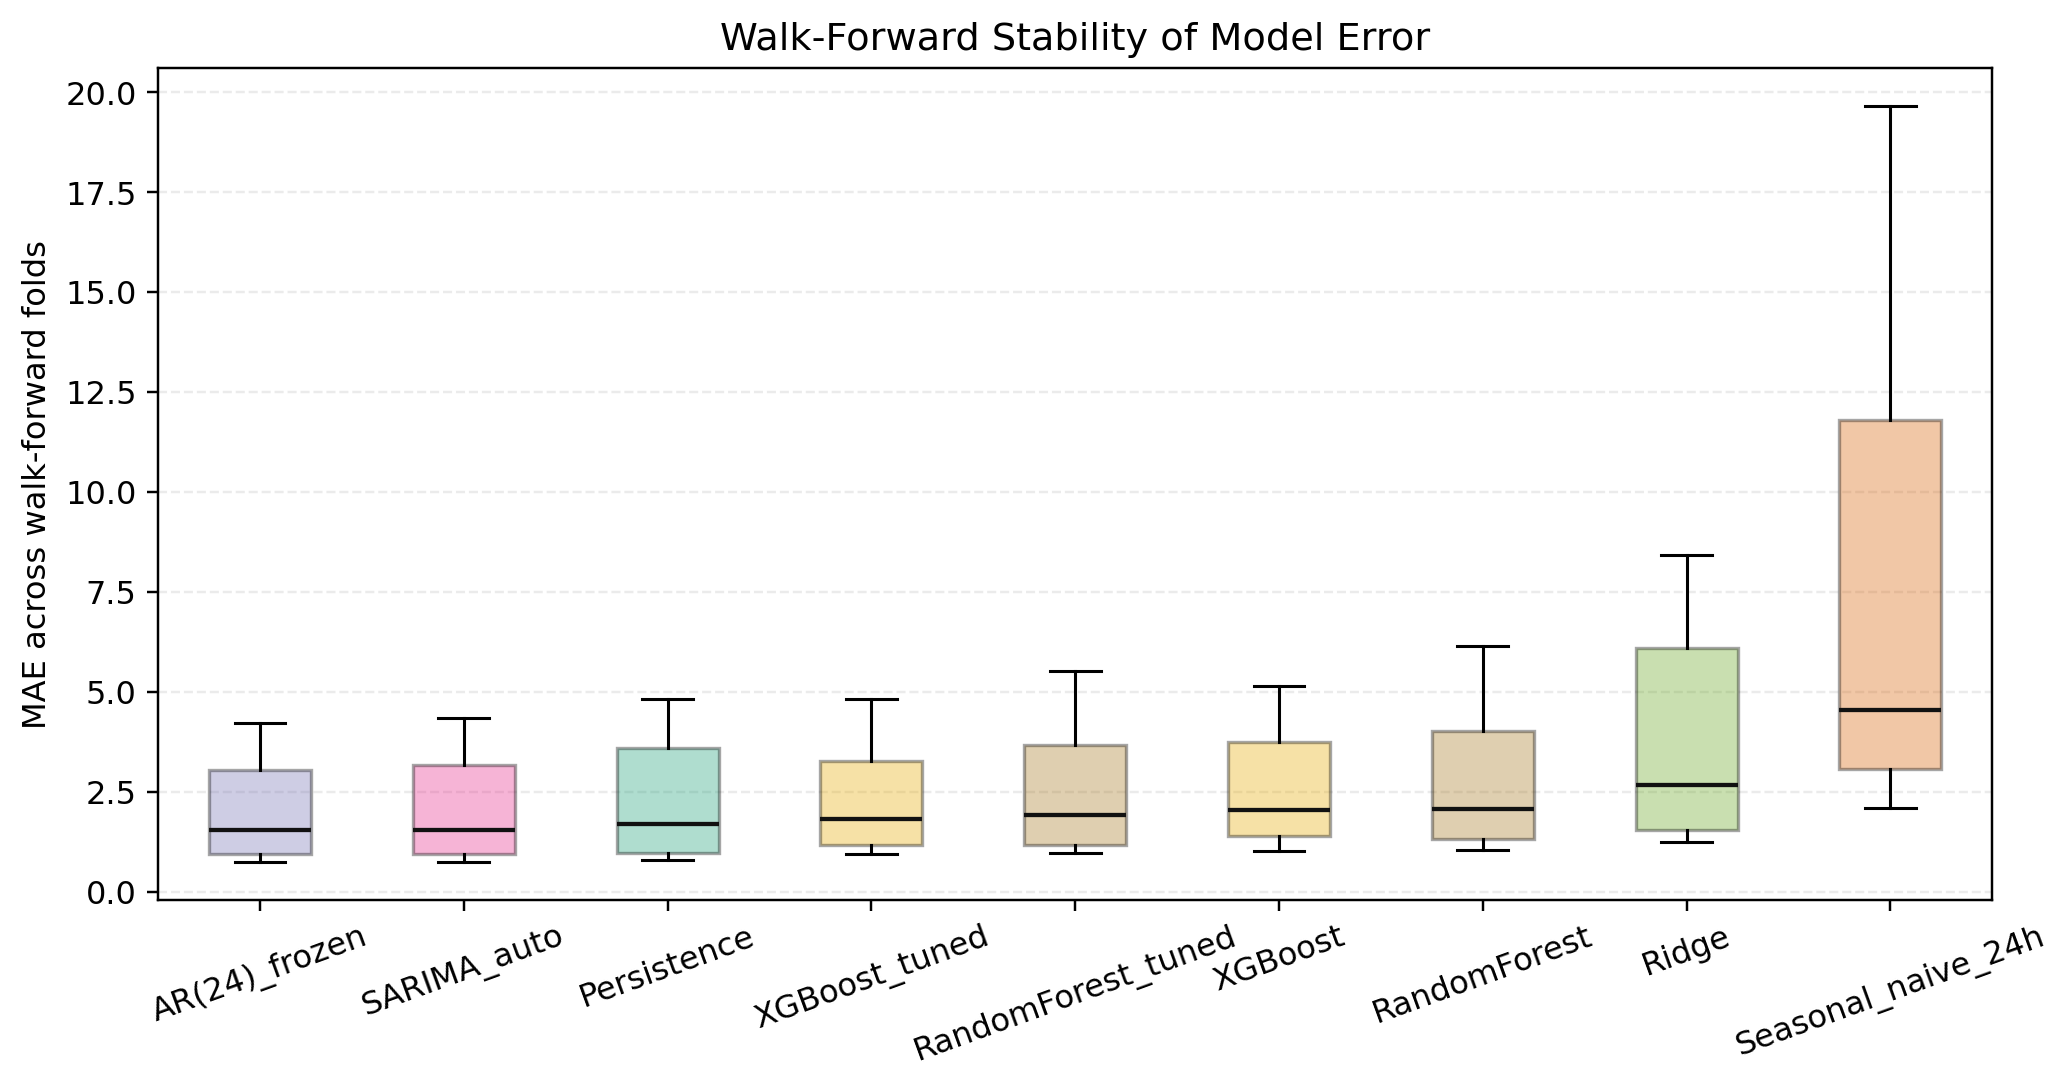
\includegraphics[width=\textwidth]{../images/walk_forward_mae_stability.png}
\end{minipage}
\caption{Left: 1-hour test MAE (horizontal extent $\propto$ MAE, rows sorted like Table~\ref{tab:main}; MAE and intervals in $\mu$g/m$^3$). For the top three models, bootstrap error bars overlap materially, indicating high variance in relative performance across episodes and weather regimes despite a clear ordering of point estimates. SARIMA at 4.38 lies above Ridge (4.66) in the vertical ordering (better MAE) and shows a \emph{shorter} bar than Ridge; Seasonal Naive (9.25) is much farther out. Right: walk-forward fold MAE stability (city mean, $\mu$g/m$^3$).}
\label{fig:spatialmae}
\label{fig:wf}
\end{figure*}

\section{Discussion and conclusion}

Strong short-lag persistence and diurnal structure make linear autoregression highly competitive on temporally honest splits; flexible ML can reduce error versus ridge yet, under our protocol, does not surpass a well-specified AR(24) on city or district-weighted 1\,h MAE (district-weighted 3.66\,$\mu$g/m$^3$ for AR(24) versus 3.82\,$\mu$g/m$^3$ for persistence). While AR(24) provides the best performance for spatially aggregated city and district metrics, simple Persistence remains the most robust baseline for individual station-level forecasting (Table~\ref{tab:spat}, Table~IV). DeepAR in our vanilla configuration remains a deliberate negative result (Table~\ref{tab:main}; MAE 26.31\,$\mu$g/m$^3$) and should not be read as a pipeline error: the failure of vanilla DeepAR is attributed to the non-stationary nature of Yerevan's winter pollution episodes, which require custom localized scaling that global sequence models lack out-of-the-box.

\textbf{Implications and future work.} For city- or district-scale indicators, long-lag AR with frozen coefficients is a strong default; fine-scale analytics may need missingness-aware weighting or spatial pooling. Reporting should always state whether metrics are computed on a spatially aggregated target or on heterogeneous stations, because the ``best'' model can change with the support even when physics does not. Probabilistic forecasts, graph models without future leakage, and nested cross-validation are natural extensions.

\textbf{Limitations.} One primary hold-out plus walk-forward analysis is not full nested cross-validation; imputation injects structured assumptions; district coverage is uneven; we estimate associations for forecasting, not causal effects. Outputs are not personal exposure estimates.

\textbf{Reproducibility.}
\ificdsgreview
Data are from the national open portal (airquality.am). Software configuration, split metadata, and extended tables are withheld for double-blind review and will be included in camera-ready and/or supplemental material.
\else
Data: national open portal (airquality.am) and repository download notes. Code: single pipeline entrypoint and paper export script in the repository; an archive script snapshots JSON and tables. Full hyperparameter tables appear in \emph{main\_long.tex} and JSON exports.
\fi

\ificdsgreview
% Acknowledgments omitted for double-blind review (ICDSG 2026).
\else
\section*{Acknowledgment}
The author thanks Rafayel Shirakyan for supervision and feedback.
\fi
\bibliographystyle{IEEEtran}
\bibliography{references}

\end{document}
